Initially, we present the statistical - and numerical methods used in the thesis. In addition, we introduce the necessary terminology and -theory from the study of dynamical systems to be able to construct our model.
\subsection{Stochastic Differential Equations}
First, we put forth the part from the general theory of stochastic differential equation that we need in order to derive estimators for the parameters of processes governed by them. 
\subsubsection{Itô integrals and - processes}
Broadly speaking a stochastic differential equation (SDE) is a generalization of a differential equation, where there is some term, which is a stochastic process. There exists many variants using different processes, yet we only consider processes driven by a Brownian motion - also known as a Wiener process. To define stochastic differential equations in this setting with more rigor we need to define a brownian motion: A brownian motion is a continuous stochastic processes, $W_t\in\mathbb{R}$ satisfying the following properties
\begin{enumerate}
    \item $X_0 = 0$ almost surely
    \item $\Delta W_n = W\left(t_{n + 1}\right) - W\left(t_{n}\right)\sim\mathcal{N}\left(0, t_{n + 1} - t_{n}\right)$
    \item $X_{t_1}\indep \left(X_{t_2} - X_{t_1}\right)\indep \dots \indep \left(X_{t_n} - X_{t_{n - 1}}\right), \: 0 < t_1 < t_2 < \dots < t_n$.
\end{enumerate}
This process is pivotal in the study of continuous-time stochastic processes. For our purposes, we define integration from $t_0$ to $t$ of some function $\sigma(X_t, t)$ with respect to $W_t$. We partition the interval $[t_0, t]$ into smaller intervals $[t_k, t_{k + 1}]$ with $t_0 \leq t_1 \leq \dots \leq t_n = t$. The integral is constructed by having the partition get increasingly finer
\begin{align}
    \int_{t_0}^t \sigma(X_s, s) \mathrm{d}W_s = \lim_{n \to \infty}\sum_{k = 0}^{n - 1} \sigma\left(X_{t_k}, t_k\right)\left(W_{t_{k + 1}} - W_{t_k}\right),\label{eq:itoIntegralDefinition}
\end{align}
where the limit is in $L_2$-sense \cite[equation 4.6]{Srkk2019}. \\
We call (\ref{eq:itoIntegralDefinition}) the Itô integral and it the central piece of Itô calculus; an area that expands the techniques of calculus to stochastic processes. Now to construct stochastic differential equations we write up the Itô integral equation
\begin{align}
    X_t - x_0 = \int_{t_0}^t b(X_s, s)\mathrm{d}s + \int_{t_0}^t \sigma(X_s, s)\mathrm{d}W_s. \label{eq:itoIntegralEquation}
\end{align}
Note that the first integral on the right hand side merely is a Riemann integral. A stochastic differential equation can then by understood by letting the limits of integration in (\ref{eq:itoIntegralEquation}) be $t$ and $t+\mathrm{d}t$ for some small $\mathrm{d}t$. That is as shorthand for (\ref{eq:itoIntegralEquation}) we may write
\begin{align}
    \mathrm{d}X_t = b(X_t, t)\mathrm{d}t + \sigma(X_t, t)\mathrm{d}W_t, \quad X_{t_0} = x_0 \label{eq:firstSDE},
\end{align}
and this is the general form of an SDE. \\
Although, the representation in (\ref{eq:firstSDE}) is the most common in the litterature and the one we use for the most part, we have to note that is merely a representation of (\ref{eq:itoIntegralEquation}). This can be seen, if we formally divide by $\mathrm{d}t$. We end up with a term, where we take the derivative of the Wiener process. This process has almost surely continuous sample paths, yet they are nowhere differentiable \cite[theorem 11.22 and theorem 11.35]{Hansen2022}.\\\\
To better understand stochastic differential equations we need to introduce a bit more nomenclature: The solution, $X_t$, is called an Itô process, and the values it can take is its state space. We refer to the functions $b(X_t, t)$ and $\sigma(X_t, t)$ as the drift- and diffusion coefficients respectively. For ease of language we sometimes leave out the "coefficient" part. In our applications the drift and diffusion depend on some parameter vector, $\theta\in\Theta\subseteq\mathbb{R}^p$. For typographical reasons though, we mostly suppress this dependence in the notation. Additionally, we say that the term with the diffusion coefficient is the noise term or stochastic term and the term with the drift is the deterministic term or deterministic part. The noise is additive, if the function $\sigma(X_t, t)$ is constant and multiplicative otherwise. Lastly, the stochastic differential equation has autonomous drift or diffusion, when they do not directly depend on time; the system as a whole is autonomous, if both parts are autonomous.\\
\\
Now, to motivate the arguably most important result in the study of stochastic differential equations, we evaluate the the Itô integral of the Wiener process
\begin{align}
    \int_0^t W_s \mathrm{d}W_s & = \lim_{n \to \infty}\sum_k W_{t_k}\left(W(t_{k + 1}) - W_{t_k}\right) \nonumber \\ 
    & = - \frac{1}{2}\lim_{n \to \infty}\sum_k \left(W(t_{k + 1}) - W(t_{k})\right)^2  + \frac{1}{2}\lim_{n \to \infty}\sum_k\left(W(t_{k + 1})^2 - W(t_{k})^2\right) \nonumber \\
    & = -\frac{t}{2} + \frac{W_t^2}{2}.
\end{align}
We have used the observation that the last sum was telescopic and equal to $W_t^2$. The first sum is the quadratic variation of the wiener process, which by \cite[theorem 11.34]{Hansen2022} is $t$.\\ Put differently, this means that
\begin{align}
    \mathrm{d}\left(\frac{1}{2}W_t^2\right) = W_t\mathrm{d}W_t + \frac{1}{2}\mathrm{d}t,
\end{align}
which is surprising, because it is not what we would expect from the normal chain rule. This means that Itô calculus needs its own version of the chain rule: Itô's formula \cite[Theorem 4.2]{Srkk2019}.  Given an Itô process, $X_t$, described by the SDE in (\ref{eq:firstSDE}) and a function $\varphi(X_t, t)$ of the process, then the Itô SDE for $\varphi$ can be computed by
\begin{align}
    \mathrm{d}\varphi(X_t, t) = \left(\frac{\partial \varphi}{\partial t} + \frac{\partial\varphi}{\partial x}b(X_t, t) + \frac{1}{2} \frac{\partial^2 \varphi}{\partial x^2}\sigma^2(X_t, t) \right)\mathrm{d}t + \frac{\partial\varphi}{\partial x}\sigma(X_t, t) \mathrm{d}W_t.
\end{align}
There are countless of important corollaries and applications of this result. The way we apply this result the most is qua the lamperti formation of a stochastic differential equation defined for an Itô process, $X_t$, given by (\ref{eq:firstSDE}) as
\begin{align}
    \psi(x, t) = \int_{\xi}^x \frac{\mathrm{d}u}{\sigma(u, t)}, \label{eq:firstLamperti}
\end{align}
for some $\xi$ in the state space of $X_t$. The lamperti-transform is obviously constructed such that $\mathrm{d}\psi(X_t, t)$ has additive noise, which is also easily verified with Itô's formula \cite[equation (7.5)]{Srkk2019}. We should be wary, though, as we have to ensure the transform is well-defined; we need to make sure we do not divide by zero in (\ref{eq:firstLamperti}). If we have a process, where this is ensured, it is called reducible. Further, to work with this in practice we define the transformed variable $Y_t := \psi(X_t, t)$; and to get the SDE in terms of $Y_t$, we thus need $\psi^{-1}$ to exist.\\\\
Finally, we note another result that is pivotal for the understanding of Itô processes. For fixed $t$, $X_t$ is a random variable, and we assume that it has some probability density, $p(X_t, t)$, with respect to the lebesgue measure. We do not work with explicitly, but it is worth mentioning that the variables are adapted to the filtration, $\mathcal{F}_n = \sigma\left(X_{t_i}: i \leq n\right)$. In addition, it each $X_t$ has some conditional density given by a previously observed variable $X_s$, $p(X_t, t | X_s, s), \; t\geq s$.\\ 
By \cite[theorem 7.1.2]{Oksendal2003_yu} all Itô processes are Markov processes, wherefore we do not need information from the entire filtration, but just the information at the present, $X_s$, to characterize the transtion completely. The transition density of (\ref{eq:firstSDE}) is given by the following partial differential equation
\begin{align}
    \frac{\partial p(X_t, t | X_s, s)}{\partial t} = -\frac{\partial}{\partial x}\left(b(X_t, t)p(X_t, t | X_s, s)\right) + \frac{1}{2}\frac{\partial^2}{\partial x^2}\left(\sigma^2(X_t, t)p(X_t, t | X_s, s)\right),\label{eq:fokkerPlanck} 
\end{align}
with initial condition $p(x_t, t|x_s, s) = \delta(x_t - x_s)$ at time $t = s$ and where $\delta$ is the dirac delta function. We refer to this PDE as the Kolmogorov forward equation. As a result of giving us the transition density the Kolmogorov forward equation lets us calculate any conditional moment, if it exists. Additionaly, it allows us to derive score-function, defined as
\begin{align}
    U(\theta; X_t, t | X_s, s) = \frac{\partial}{\partial\theta}p(X_t, t | X_s, s), \label{eq:transitionScore}
\end{align}
and this can in principle be used to derive score equations for maximum likelihood estimation. In practice, however, (\ref{eq:fokkerPlanck}) is often untractable - meaning that we are unable to find the closed form solution for the transition density and thereby also the score. In this situation, one approach we often use is to somehow approximate the transition density.\\
Closely related to these concepts is the so-called infinitesemal generator 
\begin{align}
    \mathcal{L}\varphi(x) = b(x, t) \frac{\partial\varphi}{\partial x} + \frac{1}{2}\sigma^2(x, t)\frac{\partial^2\varphi}{\partial x^2} \label{eq:infinitesemalGeneratorDefinition},
\end{align}
which is an operator on some sufficiently regular function, $\varphi$. We say that $\varphi$ and $\lambda$ are the eigen functions and -values for the process respectively, if 
\begin{align}
    \mathcal{L}\varphi = -\lambda\varphi.
\end{align} 
These objects are central in the understanding of the evolution of the solutions to the stochastic differential equation, for which we do not have the closed form solutions to (\ref{eq:fokkerPlanck}). Under mild regularity conditions \cite[theorem 1.16]{StatisticalMethodsForSDE} namely states
\begin{align}
    \mathbb{E}\left[\varphi(X_{t}) \middle | X_{s}\right] = \exp\left(-\lambda \left(t - s\right)\right)\varphi \label{eq:momentConditions}, \quad t\geq s.
\end{align}
even when we cannot find the solution to (\ref{eq:fokkerPlanck}), we still have methods to calculate the conditional moments of the eigen functions of the process.\\
As is clear, though, we need the specific eigen function to be sufficiently simple e.g. a polynomium to actually be able to calculate the specific condtional moments, we are interested in. This is typically the first and second conditional moment.
\subsubsection{The Ornstein-Uhlenbeck process}
As mentioned, closed-form solutions can only be derived for select stochastic differential equations. One such process is the Ornstein-Uhlenbeck process
\begin{align}
    \mathrm{d}X_t = -\alpha_0\left(X_t - \mu\right)\mathrm{d}t + \sigma \mathrm{d}W_t, \quad X_{t_0} = x_0. \label{eq:originalOUprocess}
\end{align}
In this rather simple process the drift and diffusion are parameterized by $\theta = \left(\alpha_0, \mu, \sigma\right)^\top$ with the constraint that $\alpha_0, \sigma>0$.
To get the closed form solution for this SDE multiply (\ref{eq:originalOUprocess}) with $\exp\left(\alpha_0 t\right)$ and rearrange
\begin{align}
    \exp\left(\alpha_0 t\right)\mathrm{d}X_t + \exp\left(\alpha_0 t\right) \alpha_0 X_t \mathrm{d}t = \exp\left(\alpha_0 t\right)\alpha_0\mu \mathrm{d}t + \exp\left(\alpha_0 t\right)\sigma \mathrm{d}W_t
\end{align}
Use Itô's formula on $\exp\left(\alpha_0 t\right)X_t$ to see
\begin{align}
    \mathrm{d}\left(\exp\left(\alpha_0 t\right)X_t\right) &= \exp\left(\alpha_0 t\right)\alpha_0 \mu \mathrm{d}t + \exp\left(\alpha_0 t\right) \sigma \mathrm{d}W_t \nonumber
\end{align}
Understanding this as the integral equation (\ref{eq:itoIntegralEquation}) yields
\begin{align}
    \exp\left(\alpha_0 t\right)&X_t - \exp\left(\alpha_0 t_0\right)x_0 = \left(\exp\left(\alpha_0 t\right) - \exp\left(\alpha_0 t_0\right)\right)\mu + \int_{t_0}^t \exp\left(\alpha_0 s\right)\sigma \mathrm{d}W_s \nonumber \\
    &X_t = \exp\left(-\alpha_0\left(t - t_0\right)\right)\left(x_0 - \mu\right) + \mu + \int_{t_0}^t \exp\left(-\alpha_0 \left(t - s\right)\right)\sigma \mathrm{d}W_s \label{eq:OU_solution},
\end{align}
which was what we wanted. Now, since the increments of the brownian motion is gaussian, the solution $X_t$ for given $t$ is gaussian. We can easily find its mean and variance using the following properties of the Itô integral \cite[theorem 3.2.1 and lemma 3.1.5]{Oksendal2003_yu}
\begin{align}
    \mathbb{E}\left[\int_{t_0}^t f(X_s, s) \mathrm{d}W_s\right] &= 0 \label{eq:meanOfItoIntegral},\\
    \mathbb{E}\left[\left(\int_{t_0}^t f(X_s, s) \mathrm{d}W_s\right)^2\right] &= \int_{t_0}^t \mathbb{E}\left[\left(f(X_s, s)\right)^2\right] \mathrm{d}s. \label{eq:ItoIsometry}
\end{align}
Taking expectation of (\ref{eq:OU_solution}) and using (\ref{eq:meanOfItoIntegral}) we get
\begin{align}
    \mathbb{E}\left[X_t\right] = \exp\left(-\alpha_0\left(t - t_0\right)\right)\left(x_0 - \mu\right) + \mu. \label{eq:OU_mean}
\end{align}
Then we take the variance of (\ref{eq:OU_solution})
\begin{align}
    \mathrm{Var}\left[X_t\right] &= \sigma^2\mathrm{Var}\left[\int_{t_0}^t \exp\left(-\alpha_0 \left(t - s\right)\right)\sigma \mathrm{d}W_s\right],\nonumber \\
    & = \sigma^2\left(\int_{t_0}^t \mathbb{E}\left[\exp\left(-2\alpha_0\left(t - s\right)\right)\right] \mathrm{d}s + 0^2 \right), \nonumber \\
    & = \frac{\sigma^2}{2\alpha_0}\left(1 - \exp\left(-2\alpha_0(t - t_0)\right)\right). \label{eq:OU_variance}
\end{align}
Where we use both (\ref{eq:meanOfItoIntegral}) and (\ref{eq:ItoIsometry}) in the second step. Note that $\alpha_0 > 0$, we see that (\ref{eq:meanOfItoIntegral}) goes to $\mu$, when $t$ goes to $\infty$. This phenomenon is called mean-reverting. There are a lot of other Itô process that have this property; and as we will see, it stems from the structure of the drift. Also, for the same reasons (\ref{eq:OU_variance}) goes to $\frac{\sigma^2}{2\alpha_0}$.
\subsubsection{Pearson diffusions}
A special family of one-dimensional Itô processes are the Pearson diffusions. Structurally, they are very similiar to the Ornstein-Uhlenbeck process in the way that they share drift function; as we will see this means that they are mean-reverting as well. More specifically, we define a pearson diffusion as a solution to a stochastic differential equation on the form
\begin{align}
    \mathrm{d}X_t = -\alpha_0 \left(X_t - \mu\right)\mathrm{d}t + \sigma\sqrt{\left(aX_t^2 + bX_t + c\right)}\mathrm{d}W_t, \: \alpha_0, \sigma > 0. \label{eq:pearsonDiffusion}
\end{align}
For appropriate choices of $a, b, c$ making the square-root well-defined in the state space of $X_t$. Our focus is on the ergodic pearson diffusions; one can show that this is a class of six special diffusions \cite[p.36]{StatisticalMethodsForSDE}. \\
Amongst other things, we consider the Lamperti-transform defined in (\ref{eq:firstLamperti}). Here, it is
\begin{align}
    Y_t := \psi\left(X_t, t\right) = \int_{\xi}^{X_t} \frac{\mathrm{d}x}{\sqrt{\left(ax^2 + bx + c\right)}}. \label{eq:lampertiDefinition}
\end{align}
Again, for some appropriate $\xi$ in the state space of the respective processes. To see that $\mathrm{d}\psi\left(X_t, t\right)$ has additive noise, we present the its SDE, derived using Itô's formula
\begin{align}
    \mathrm{d}\psi\left(X_t, t\right) = - \frac{1}{\sqrt{\left(aX_t^2 + bX_t + c\right)}}\left(\alpha_0\left(X_t - \mu\right) + \frac{\sigma^2}{4}\left(2aX_t + b\right)\right)\mathrm{d}t + \sigma \mathrm{d}W_t.
\end{align}\\
However, to get the expression of $\mathrm{d}Y_t$ we have to invert $\psi\left(X_t, t\right)$ and this is obviously not possible in the general case of (\ref{eq:lampertiDefinition}); it needs to be handled casewise.\\
We sketch a quick overview of the processes \cite[p.36]{StatisticalMethodsForSDE} and their lamperti-transform\\\\
\begin{table}[h!]
    \begin{center}
    \begin{tabular}{lllll}\hline
    \textbf{Name} & \textbf{Diffusion term} & \textbf{Lamperti-transform} & \textbf{State space}\\ \hline
    Ornstein-Uhlenbeck  & $\sigma$  & $X_t$ & $\mathbb{R}$ \\
    Square-root process & $\sigma\sqrt{X_t}$  & $ 2\sqrt{X_t}$ & $\mathbb{R}_{>0}$ \\
    Mean-reverting GBM  & $\sigma X_t $  & $ \log\left(X_t\right)$  & $\mathbb{R}_{>0}$ \\
    Skew t-diffusion  & $\sigma\sqrt{X_t^2 + 1}$  & $ \sinh^{-1}(X_t)$ & $\mathbb{R}$\\
    Scaled F-diffusion  & $\sigma\sqrt{X_t\left(X_t + 1\right)}$  & $ 2\sinh^{-1}\left(\sqrt{X_t}\right)$ & $\mathbb{R}_{>0}$ \\
    Jacobi-diffusion  & $\sigma\sqrt{X_t\left(1 - X_t\right)}$  & $ 2\sin^{-1}\left(\sqrt{X_t}\right)$ & $(0, 1)$ \\ \hline
    \end{tabular}
    \caption{Overview of the ergodic pearson diffusions}
    \label{table:ergodicDiffusions}
\end{center}
\end{table}\\
For the the expressions of $\mathrm{d}Y_t$ for each of the diffusions refer to appendix \ref{sec:AppendixEstim}. If we consider the diffusion terms in table \ref{table:ergodicDiffusions}, it is clear that (\ref{eq:lampertiDefinition}) is always well-defined; that is, the processes are reducible. Additionally, we see that the respective lamperti-transform are one-to-one on the state space and therefore have well-defined inverse. \\\\
In spite of not being specifically important for our purposes, we note that although named the erdogic pearson diffusions, some are not ergodic for any choice of parameters. Whether there are any conditions for ergodicity and what these are depends on the diffusion in question; the condition, of course, is on the parameters. For instance, the Ornstein-Uhlenbeck is always ergodic and has invariant distribution $\mathcal{N}\left(\mu, \frac{\sigma^2}{2\alpha_0}\right)$, whereas the square-root process is ergodic if and only if $2\alpha_0\mu\geq \sigma^2$ with invariant distribution $\Gamma\left(\frac{2\alpha_0\mu}{\sigma^2}, \frac{2\alpha_0}{\sigma^2}\right)$. \\
Yet, more beneficial for our applications is the fact that Forman and Sorensen \cite{FormanSorensen2008} proved that for our ergodic diffusions, the eigen functions are all polynomials. Because of this, we can use (\ref{eq:momentConditions}) to derive any conditional moment of these processes, in spite of the fact that the transition densities themselves, for the most part, are unknown. Still, the calculations can become quite involved algebraically; this is especially true for moments of higher order. For this reason, we only used the first two eigenfunctions and eigenvalues: those associated with the first- and second-order polynomials. To this end, observe that regardless of the noise term, (\ref{eq:pearsonDiffusion}) always have the same first-order eigen function and eigen value, due to the vanishing of the noise term in (\ref{eq:infinitesemalGeneratorDefinition}), whenever $\varphi$ is affine. This naturally results in the same conditional mean too, which for any of the diffusions in table \ref{table:ergodicDiffusions} is
\begin{align}
    \mathbb{E}\left[X_{t_{i}+\Delta} \middle|X_{t_{i}} \right] = \exp\left(-\alpha_0\Delta t\right)\left(x-\mu\right) + \mu
\end{align}
This we also verify directly for a concrete pearson diffusion in (\ref{eq:directVerificationCondMean}). Though, it is evident that the calculations are completely analagous for the other pearson diffusions. We regognize the mean-reverting nature of the conditional moments that the moment of the OU-process had. With regard to the the conditional second moments and -variances, however, we need to consider the processes individually.
\subsubsection{Discretization of stochastic differential equations}\label{subsubsec:Discretization}
In their abstract form stochastic differential equation are inherently different to the actual observations from them in real world applications.
When sampling or considering sample paths from stochastic differential equations we are naturally limited to a finite amount of samples. Typically, we are in a situation, where we have samples $X_{t_0},\dots,X_{t_n}$ for some times $t_0,\dots,t_n$. We denote the time between the observations the temporal resolution of the data write $\Delta t_i = t_{i} - t_{i - 1}$; this quantity is for simplicity often constant and when it is, we refer to it as uniform temporal resolution. Given the sample from data, we can just use the markov property and the methods that stem for it, to do inference. If we on the other hand, want to draw samples from an SDE such as  (\ref{eq:firstSDE}), we need to use a different idea. 
\subsection{Dynamical systems}
When studying a system that evolves over time, one thing that frequently interests us is the long-term behaviour of the system: Will it reach an equillibrium of sorts, oscillate or something completely different. Answers to these types of questions are what we call the systems dynamics. The type of dynamics we are concerned with are the differential equation type of dynamical systems. Initially, we introduce relevant terminology for dynamical systems in their classic deterministic setting; then we see that they also align well in the setting of stochastic differential equation. 
\subsubsection{Deterministic Dynamical Systems and bifurcations}
A general dynamical system can be written as
\begin{align}
    \mathrm{d}x_t = f(x_t, \lambda)\mathrm{d}t, \label{eq:generalDynamicalSystem}
\end{align}
where $x_t$ is some variable of interest and $\lambda$ is a parameter that, for now, is fixed. In physics, these systems often understood as changes to a so-called potential, $V(x,\lambda)$, used to model numerous physical phenomena. That is, 
\begin{align}
     f(x_t, \lambda) = \left.-\frac{\partial V(x,\lambda)}{\partial x}\right|_{x=x_t}
\end{align}
We frequently describe the system by refering to its flow. The flow is to the right, when $f(x_t, \lambda)$ is positive; and to the left, if it negative. In the case, when $f(x_0, \lambda) = 0$, the point $x_0$ is called a fixed point. The fixed point is stable, if $\frac{\partial}{\partial x}f(x_0, \lambda) < 0$ and unstable, if it is positive. In the last instance, we say it is half-stable. From which direction the fixed point is unstable and stable depends on the second derivative of $f$.
As an example consider the double-well potential
\begin{align}
    V(x,\lambda) = \frac{x^4}{4} - \frac{x^2}{2} + \lambda x\label{eq:doubleWellPotential}.
\end{align}
By definition, this potential models the following dynamical system
\begin{align}
    \mathrm{d}x_t = f_{DW}(x_t, \lambda) = \left(-x_t^3 + x_t - \lambda \right) \mathrm{d}t \label{eq:originalDW}.
\end{align}
We depict this model for a few values of $\lambda$
\begin{figure}[h]
    \begin{center}
        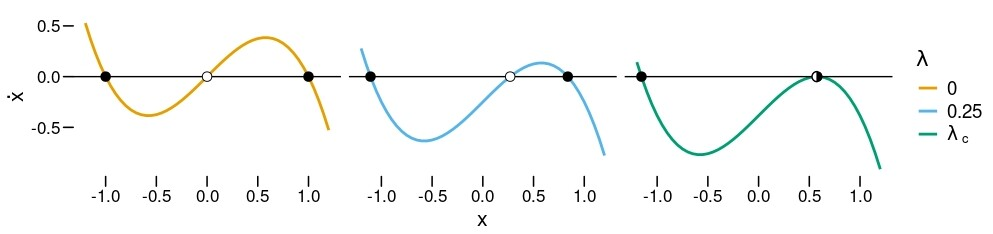
\includegraphics[scale = .5]{figures/double_well_plot.jpeg}
        \caption{The flow of the DW-potential dynamical system for varying values of $\lambda$.}
        \label{figure:DW_dynamic_plot}
    \end{center}
\end{figure}\\
In the intercepts we have the fixed points. By convention fixed points are marked as points. Stable fixed points are solid points, whereas unstable are hollow. This is easily seen by simply looking at the graphs. Recall that when $\dot{x}_t$ i.e. $x_t'$ is below 0, the flow is to the left and vice versa. Now, we notice something interesting with the value $\lambda = \lambda_c$; the numeric value of which we have suppressed in the plot. The system goes from having three fixed points: Two stable and one unstable, to just two fixed points: One stable and one half-stable. Mathematically, there is a real double root at that point, and looking at the graph it is clear that this change in $\lambda$ results in a rather different qualitative behaviour of the system. From the definition it is not difficult to see that increasing the value further would leave the system with just one stable fixed point. This type of change in the characteristics of a dynamical system, we call a bifurcation. And the values, $\lambda_c$, for which the changes occurs, we refer to as bifurcation points.\cite{Strogatz2019_gv}. In applications, these points are also sometimes refered to as tipping points and the phenomenon as tipping\\
To get an understanding of why this happens, we need to compute the cubic discriminant. For a cubic polynomial in depressed form such as the dynamic (\ref{eq:originalDW}), we can compute this quantity as
\begin{align}
    \Delta_{\mathrm{DW}} = -\left(4(-1)^3+27\left(\lambda\right)^2\right) = -27\lambda^2 + 4. \label{eq:DW_discriminant}
\end{align} 
Whenever the result is positive; there are three solutions, when it is zero, there are two solutons. Finally, for negative values, there is only one solution to the cubic polynomial. The discriminant is a second degree polynomial in the parameter $\lambda$ and it has roots $\pm \frac{2}{3\sqrt{3}}$. The system depicted in figure \ref{figure:DW_dynamic_plot} uses the positive root for the graph depicted with $\lambda_c$. Yet, it is not difficult to imagine that decreasing the value of $\lambda$ would result in a mirrored, but completely analagous qualitative change to the one we observe in figure \ref{figure:DW_dynamic_plot}. Mathematically, this is due to $\Delta_{\mathrm{DW}}$ being positive between the two roots and negative outside. In the following, we focus on the positive root; though it should be noted that our reasoning is not limited to this bifurcation point. $\lambda_c$ and the half-stable fixed point pertaining to it constitute an example of a specific type of bifurcations known as saddle-node bifurcations. For this value of $\lambda_c$ the stable fixed point is found at $x_1^* = -\frac{2}{\sqrt{3}}$, and the half-stable is $x_2^* = \frac{1}{\sqrt{3}}$. We study the behaviour of the system close to the pair $(x, \lambda) = (x_2^*, \lambda_c)$. A taylor expansion of $f_{\mathrm{DW}}$ to the second order around the x-value and first order around the $\lambda$-value gives the following
\begin{align}
    f_{\mathrm{DW}}(x_t,\lambda)&\approx \frac{\partial}{\partial x_t}f_{\mathrm{DW}}(x_2^*,\lambda_c)(x-x_2^*) + \frac{1}{2}\frac{\partial^2}{\partial x_t^2}f_{\mathrm{DW}}(x_2^*,\lambda_c)(x_t-x_2^*)^2 \nonumber \\
     &+ \frac{\partial}{\partial \lambda}f_{\mathrm{DW}}(x_2^*,\lambda_c)(\lambda - \lambda_c) = -\sqrt{3}\left(x_t-x_2^*\right)^2 - \left(\lambda - \lambda_c\right) \nonumber \\&= -\left(\tilde{x}_t^2 + \tilde{\lambda}\right), \label{eq:prototypicalSaddleNode}
\end{align}
where $\tilde{x}_t = 3^{\frac{1}{4}}\left(x_t-x_2^*\right)$ and  $\tilde{\lambda} = \lambda - \lambda_c$. That is for values close to the bifurcation point the dynamic behaves similarly to that of this function, which is a quadractic polynomial in $x$ and linear in $\lambda$. Not only, is it a quadratic is $x$, it is also a rather simple quadractic with linear and intercept terms equal to zero. With $x_2^*$ being a fixed point, this was expected for the intercept. However, that the derivative of $f_{\mathrm{DW}}$ also evaluated to zero was not obvious. In fact, systems with bifurcations that locally around its bifurcation point behave in this way are what we understand by systems with saddle-node bifurcations. It is clear that any system that taylor-expands in this manner has this behaviour. That is close to the bifurcation, the dynamics will roughly look like that of (\ref{eq:prototypicalSaddleNode}). For this reason, these dynamics are what is known as prototypical- or normal forms of the saddle-node bifurcation. Doing similar calculations for (\ref{eq:DW_discriminant}), will reveal that the prototypical form in complete generality is
\begin{align}
    \mathrm{d}x_t = \pm\left(x_t^2 + \lambda\right)\mathrm{d}t
\end{align} 
As we see in the calculatation of (\ref{eq:prototypicalSaddleNode}), these forms do not care about scaling and shifting, whence we write the normal form as
\begin{align}
    \mathrm{d}x_t = \pm\left(A\left(x_t - m\right)^2 + \lambda\right)\mathrm{d}t, \label{eq:standardform}
\end{align}
where $A>0$. Note that $x_t$ is not the same as the one from the double-well potential from earlier; we live with this ambiguity to avoid introducing too much notation.\\ In sum, we have illustrated that for some systems, which change qualitative behaviour at some parameter values, the flow is approximated by what we refered to as the normal form. Studying (\ref{eq:standardform}) system, we first note that is has quadratic discriminant $\Delta_{\mathrm{sf}} = -4A\lambda$. That is, we have two solutions to \ref{eq:standardform}, i.e. the system has two fixed points, whenever $\lambda<0$, one fixed point for $\lambda = 0$ and zero otherwise. When they exist, the fixed points are given by
\begin{align}
    \mu\left(\lambda\right) = m \pm \sqrt{-\frac{\lambda}{A}}, \label{eq:fixedPoint}
\end{align}
there is one stable- and one unstable fixed point, when $\lambda<0$ and one half-stable when $\lambda=0$. Which of the two is stable and vice versa depends on the sign of the normal form \ref{eq:standardform}. Instead of illustrating the bifurcation qua the flow graph, we depict the phenomenon with a so-called bifurcation diagram\\
\begin{figure}[h]
\begin{center}
    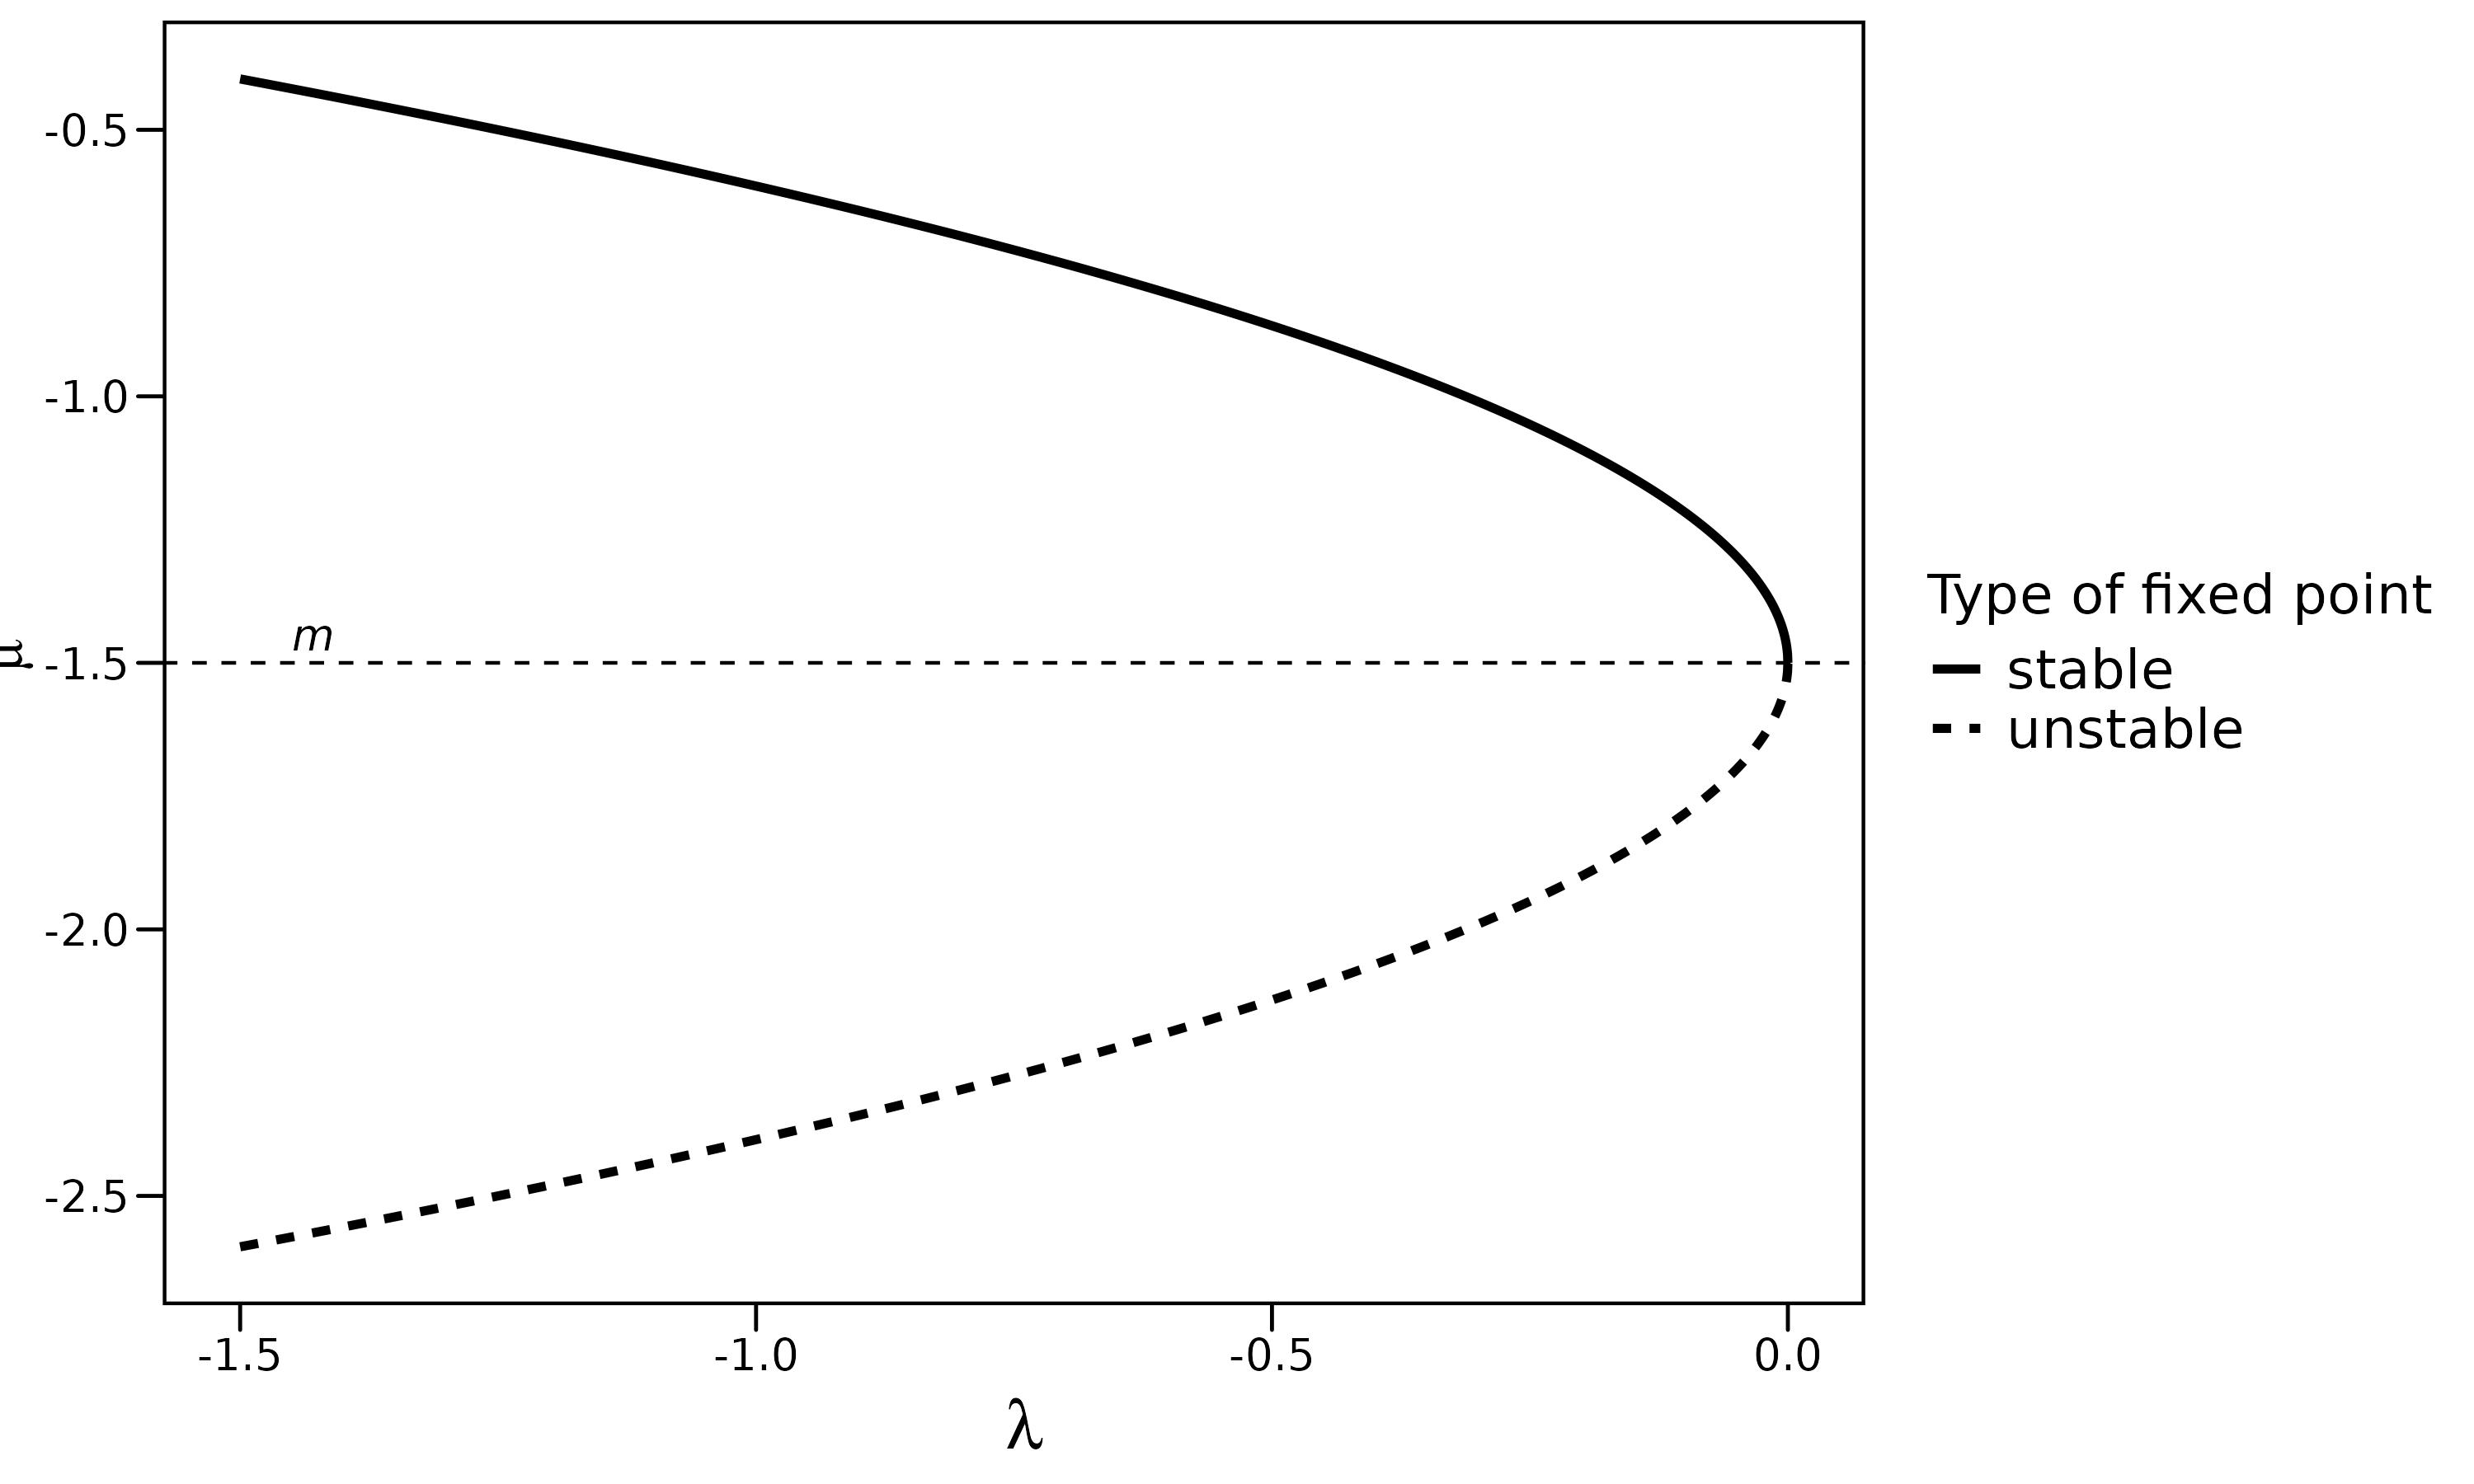
\includegraphics[scale = .4]{figures/bifurcation_diagram.jpeg}
    \caption{Bifurcation diagram of the scale and shifted normal saddle-node bifurcation.}
    \label{figure:bifurcationDiagram}
\end{center}
\end{figure}\\
Note that for $A$ and $m$ we picked $0.8$ and $-1.5$ respectively. The bifurcation diagram in figure \ref{figure:bifurcationDiagram} are the epitome of such diagrams for systems with a saddle-node bifurcation. As we have illustrated, any system with this type of bifurcation will eventually resemble (\ref{eq:standardform}) and hence their bifurcation diagram will too. One can also do the computations for the other branch of the normal form. In this case the fixed points in the bifurcation diagram are the same as before barring the fact that the types of the fixed points are swapped, i.e. for this system figure \ref{figure:bifurcationDiagram} would be mirrored around $m$.
\subsubsection{Tipping points}
We are now equipped with the necessary vocabulary to understand the model with which we estimate tipping points. We are unaware of the overall system dynamics, for which we wish to estimate tipping. However, we assume that the system has a saddle-node bifurcation. Thus, we know that sufficiently close to the bifurcation point, we can consider the scaled and shifted prototypical saddle-node bifurcation system (\ref{eq:standardform}) in the general system's stead. For fixed $\lambda < 0$ in (\ref{eq:standardform}) the system is overall stable and will converge to the stable fixed point, when we are not too far away from it. However, for values on the other side of the unstable fixed point, the values diverge to infinity. Now, imagine we are in the negative branch of (\ref{eq:standardform}). As can be seen in the graph, the system diverges when there are two fixed point and the process finds itself below the unstable fixed point. However, whenever $\lambda>0$ the system always diverges. To estimate a tipping point is to estimate a point in time, when this changes in characteristic of the system begins. We will do so by modelling a ramping of $\lambda$ from some base value $\lambda_0$ it finds itself in, when the system is overall stable. We imagine that when we have observed the system for some time, $t_0$, it is disturbed or altered in some way that begins the ramping. There are several different ways this can be modelled, but here we let $\lambda$ depend on time, $t$ in the following way
\begin{align}
    \lambda_t = \lambda_0\left(1 - \max\left\{\frac{t - t_0}{\tau_c},0\right\}\right)^\nu, \label{eq:lambdaRampDefinition}
\end{align} 
which is the model from \cite[equation (2)]{Ditlevsen2023} with the addition of the parameter, $\nu>0$. As said $t_0$ can be understood as the time when ramping of $\lambda_t$ starts. The parameter $\tau_c$ is the amount of time after ramping begins for $\lambda_t$ to become zero. This is the point, when the fixed points in \ref{figure:bifurcationDiagram} become one. That is, the point the model says that the dynamics of the system changes significantly: The tipping point. \\Now, it is crucial to understand that the normal form is only a good approximation for a system with a saddle-node bifurcation close to its bifurcation point. Far from the tipping point or after the system has tipped and the dynamics of the normal form are no longer a good approximation of the dynamics of the real system. Put differently, our model does not allow us to interpret the system after it has tipped and we need to ensure that we observe it close enough for the dynamics to be close to the normal form. How close to the bifurcation point we need to be depends on the system at hand. More positively, our models simplicity is striking. We can be completely agnostic about the actual dynamics of the system, we are considering, when our main interest is the behaviour close to- or at the bifurcation point. As long as they have a saddle-node bifurcation, these dynamics could be arbitrarily complex, so (\ref{eq:standardform}) is potentially a huge simplification.
\subsubsection{Tipping in stochastic systems}
As is done in \cite[equation (1)]{Ditlevsen2023}, we introduce noise into the normal form (\ref{eq:standardform}) to model the various uncertainties in the system. To reiterate from our introducing of stochastic differential equations, this results in a shift in the understanding of $X_t$. Now, for each point in time, $t$, the solution, $X_t$ to the noisy standard form has some distribution. Instead of only additive noise, though, we model the stochastic term as having the same noise as one of the pearson diffusions (\ref{eq:pearsonDiffusion}). In sum, the model we consider is
\begin{align}
    \mathrm{d}X_t = \pm\left(A\left(X_t - m\right) + \lambda_t\right)\mathrm{d}t + \sigma\sqrt{\left(aX_t^2 + bX_t + c\right)}\mathrm{d}W_t, \label{eq:standardStochasticForm}
\end{align}
with $\lambda_t$ given by (\ref{eq:lambdaRampDefinition}). Note that the constants: $a, b$ and $c$ are picked such that the square-root is well-defined. In particular, we use the noises from the ergodic pearson diffusions from table \ref{table:ergodicDiffusions}. For clarity, $W_t$ is a brownian motion, which we defined in the beginning, ergo the solution to (\ref{eq:standardStochasticForm}) is an Itô process. Extending dynamical systems in this manner is commonplace in various applied settings such as physics or finance. Typically, one models the overall and well understood dynamics of the system via the deterministic term. Then introducing a stochastic term into the dynamics lets us model the fact that there are parts of the system we do not understand and cannot model directly via deterministic dynamics, or alternatively that the measurements we have are inaccurate or noisy in some manner. Using the sampling scheme described in section (\ref{subsubsec:Discretization}) we draw three sample paths with the same realizations of $W_t$ for each of the models to illustrate how they differ. One row will correspond to one path. The model we use is the one with a negative sign in front of the drift in (\ref{eq:standardStochasticForm})
\begin{figure}[h]
    \begin{center}
        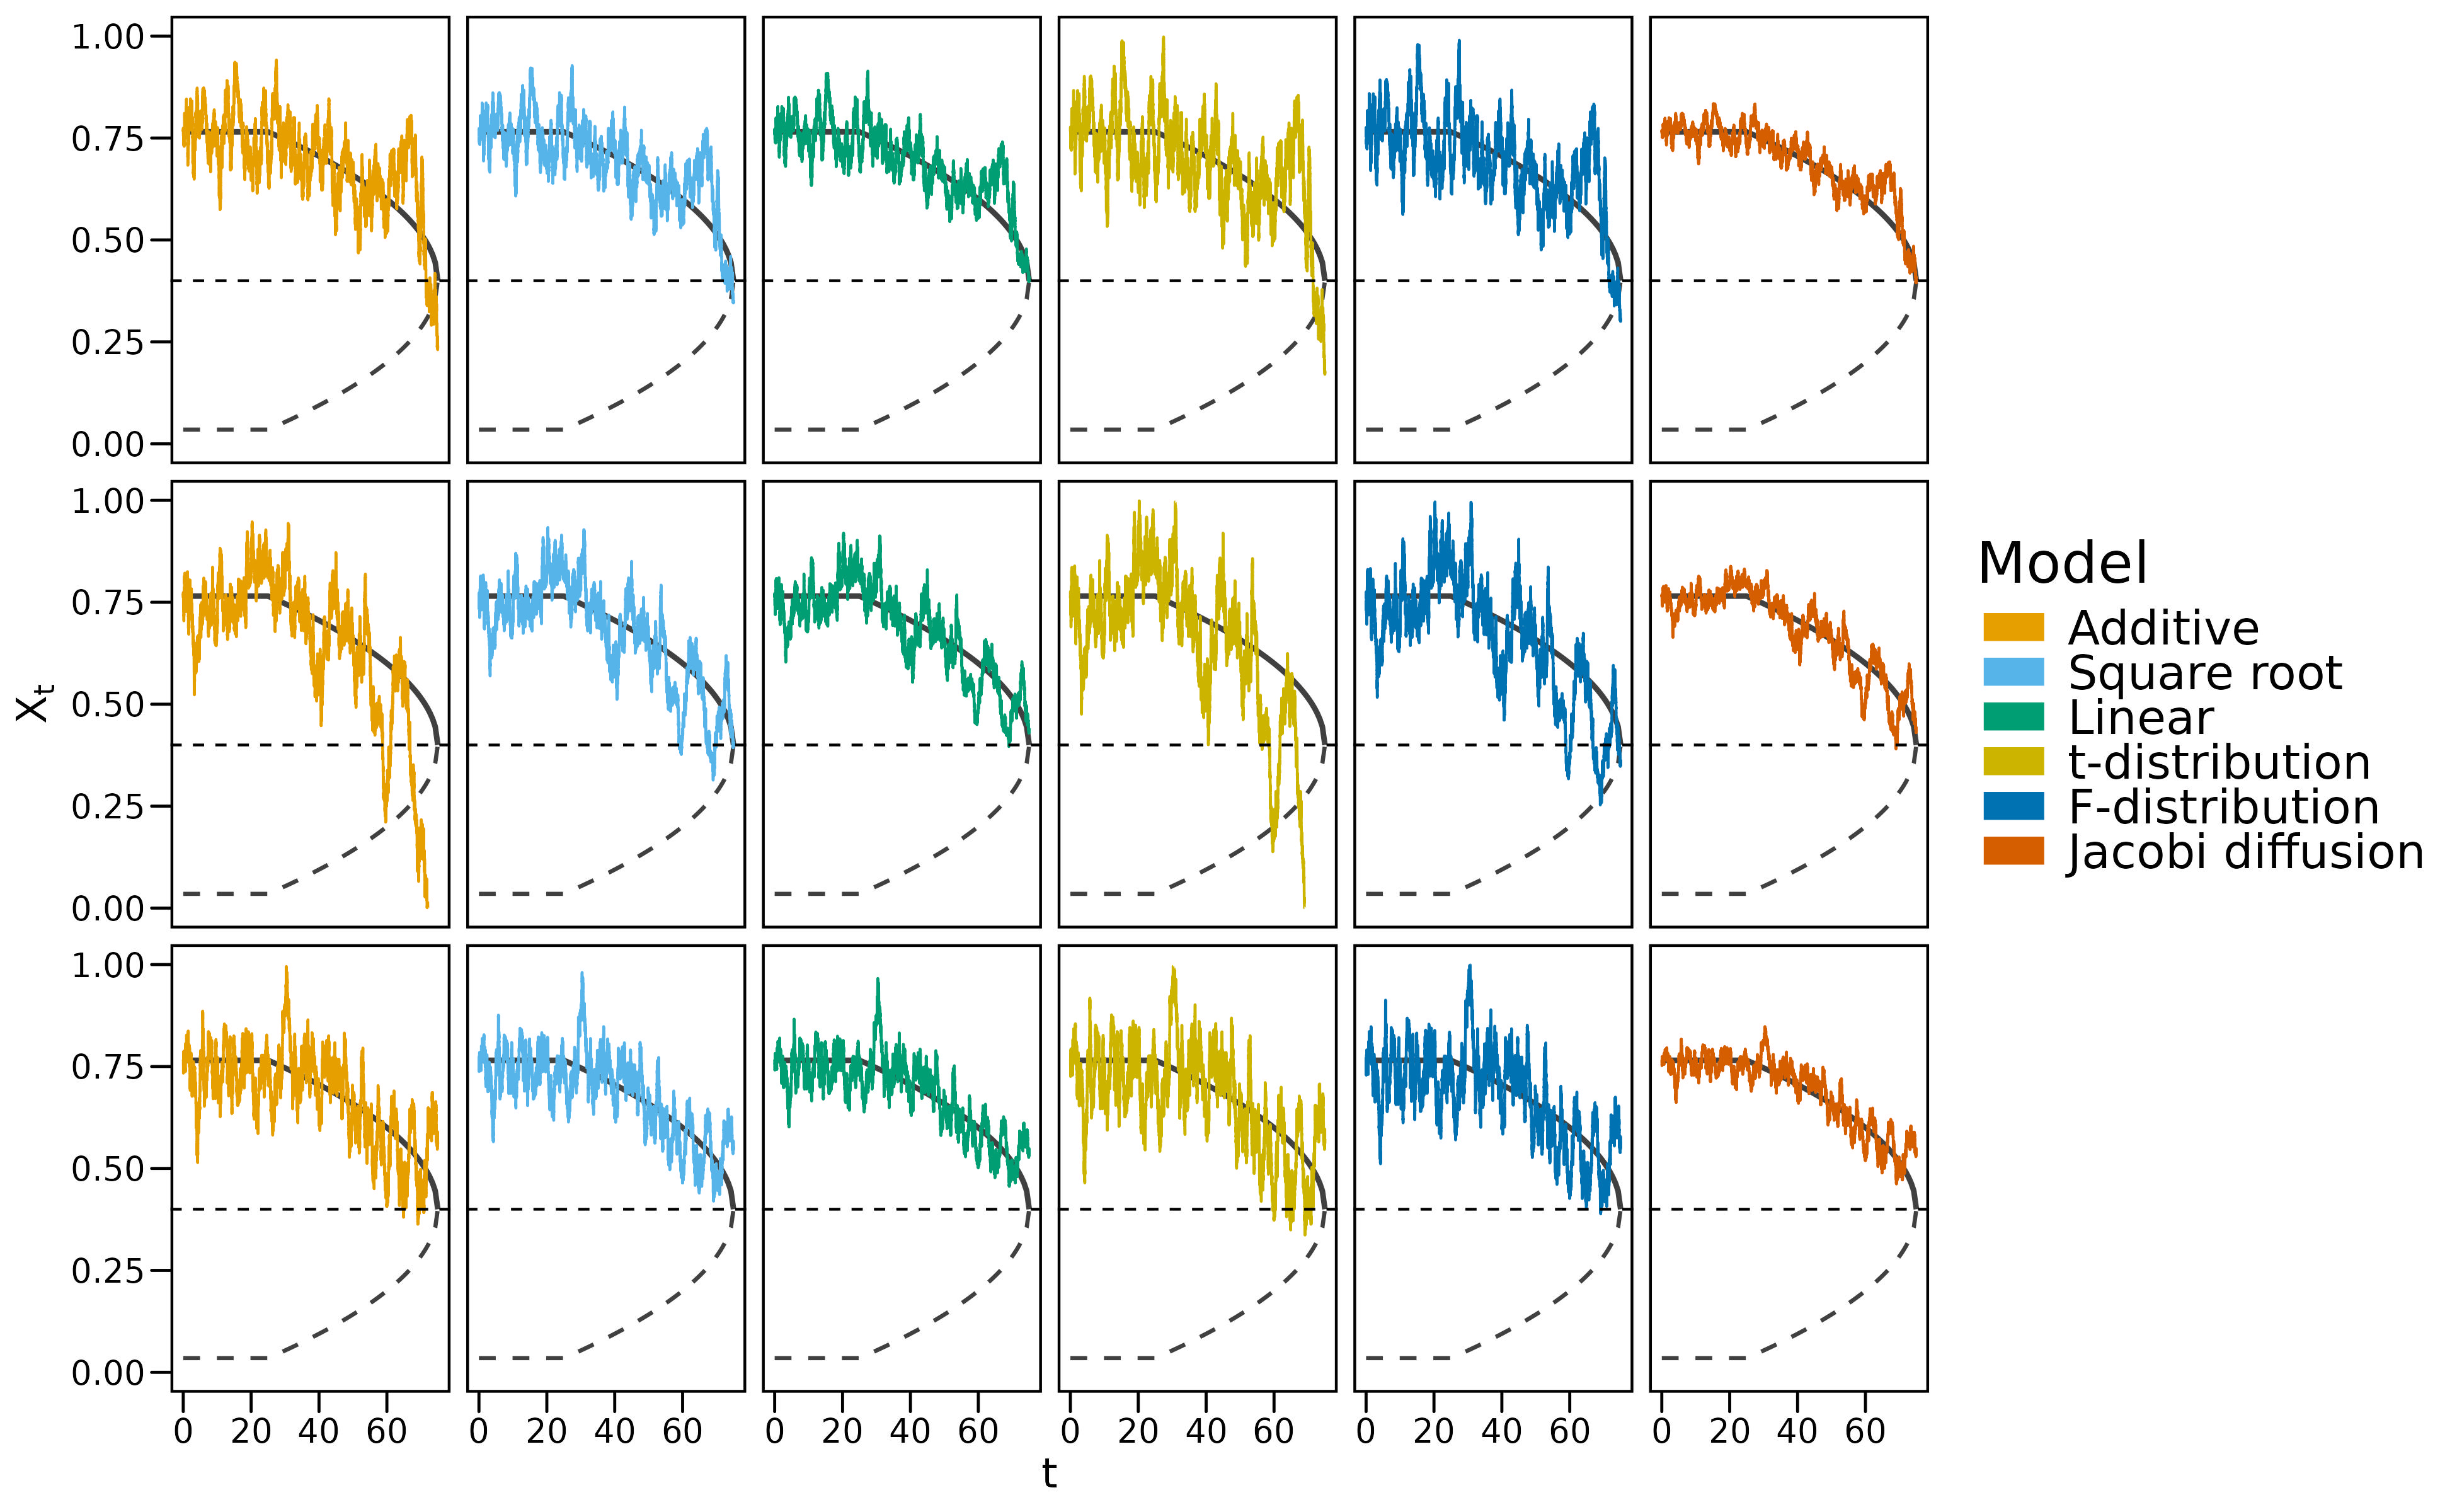
\includegraphics[scale = .1]{figures/sample_paths_plot_small_scale.jpeg}
        \caption{The dynamics of (\ref{eq:standardform}) with the six different noise terms from table (\ref{table:ergodicDiffusions}) applied to the same three realizations of a brownian motion.}
        \label{figure:samplesFromAllDifferentModels}
    \end{center}
\end{figure}\\
All the samples were drawn with parameters, $A = 1.5, m = 0.4, \lambda_0 = -0.2, \sigma = 0.1$ and $\nu = 1$. These parameters are carefully selected to ensure that we are in the state space of all processes in table \ref{table:ergodicDiffusions}. The process is started at time $0$ in its stable fixed point and starts ramping at $t_0 = 25$. The bifurcation point was set at time $75$, which means that $\tau_c = 50$. In sum, this means that in accordance with (\ref{eq:fixedPoint}) and (\ref{eq:lambdaRampDefinition}) the stable and unstable fixed points start moving from $m\pm\sqrt{\frac{\lambda_0}{A}}$ at time $t_0$ toward $m$ at time $t_0 + \tau_c$. Similarly to figure (\ref{figure:bifurcationDiagram}) this is depicted using a solid and dashed line respectively. The smaller horizontal dashed line they meet at is naturally, $m$. This is the effect of the specific form of ramping in (\ref{eq:lambdaRampDefinition}), i.e. a square-root evolution of the fixed points towards $m$ at the tipping point. This is the model from \cite{Ditlevsen2023}. Regardless of the noise, all the models have a bifurcation tipping at time $t_0+\tau_c$ the point, we have simulated up to. However, due to the random nature of the brownian motion in the stochastic term not all models tip at that point. As we discussed with regards to figure \ref{figure:bifurcationDiagram}, the deterministic part of the process will diverge below the unstable fixed point. We see that the additive noise model as well as the model with stochastic term from the ergodic diffusion with the $t$-distribution as its stationary distribution, cross the unstable fixed point prematurely twice. This phenomenon is called noise induced tipping and is exclusively a phenomenon in the study of dynamic system with stochastisity. All of the models are, in principle, always able to tip via noise. Still, for this to have any significant chance of happening the noise has to be on a scale that compares with the jump the process needs to make. In our case, this jump is the distance between the stable- and unstable fixed points at any given time point. However, the closer the path gets to the bifurcation point, the smaller the jump has to be. This is also why, we actually see the square-root- and linear noise based models along with the model that has the same noise as the diffusion with the scaled $F$-distribution. Now, from table \ref{table:ergodicDiffusions} it is clear that the model with the same noise as the diffusion with the $t$-distribtion as its stationary distribution will always have larger diffusion term than the model with additive noise. Thus, if the additive noise model has noise-induced tipping, then so will the $t$-diffusion based model. This difference will be even more pronounced when the scale is further away from zero. This is also true for some of the other models. In figure \ref{figure:samplesFromAllDifferentModels} we have chosen parameters such that we are on the unit interval. This is to accomodate for the relatively specific state space of the jacobi-diffusion based model. If we disregard this model, all the processes are well-defined on at least the positive reals. To illustrate what role the scale of our observations plays on the noise terms in the models. We use the same Wiener realizations as earlier, although we only use the first two for this example. We depict the paths with the same $t_0, \tau_c, \sigma, A$. This time, though, $m = 3$ and $\lambda_0 = -1.75$ to shift the process away from the unit interval. We get the following results
\begin{figure}[h]
    \begin{center}
        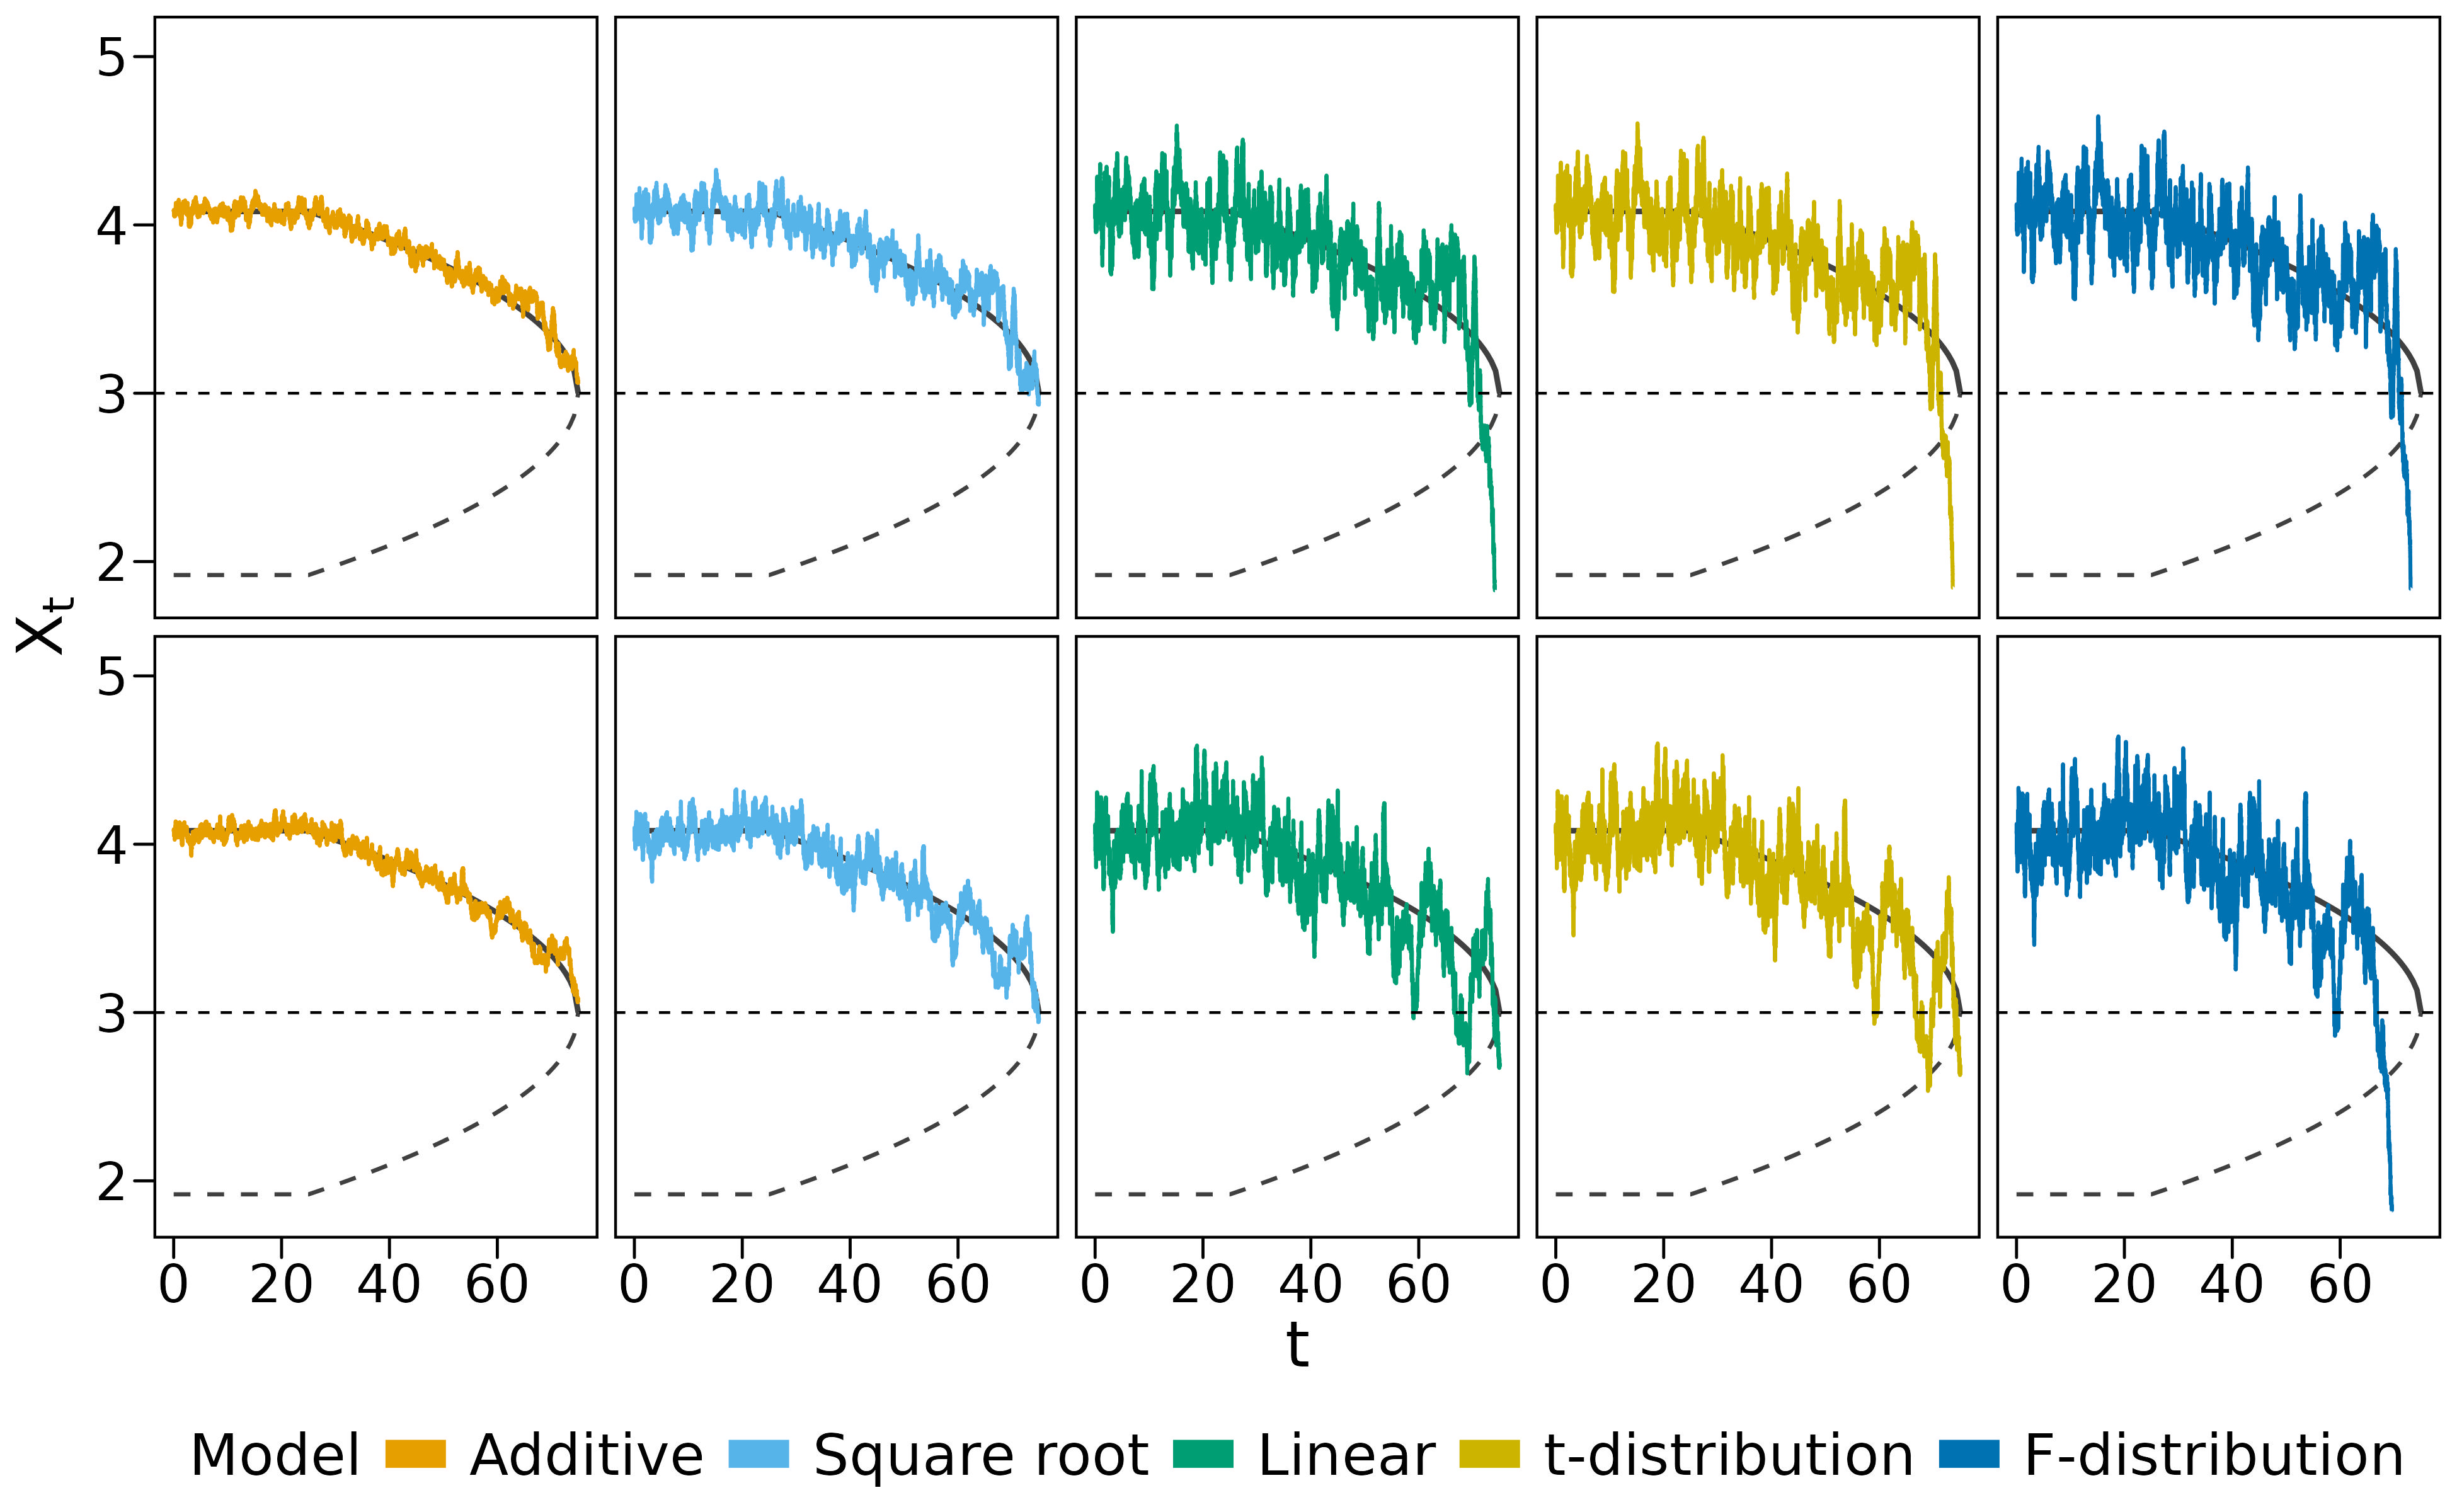
\includegraphics[scale = .1]{figures/sample_paths_plot_big_scale.jpeg}
        \caption{The dynamics of (\ref{eq:standardform}) shown on a different scale than figure \ref{figure:samplesFromAllDifferentModels} but with the same realizations of the Wiener process.}
        \label{figure:samplesFromFiveDifferentModels}
    \end{center}
\end{figure}\\
Nevertheless, it is evident that the these models are parametric. For us to do any inference on them, we need to be able to parameter estimation in stochastic differential equation, which is something we have yet to introduce. 
\newpage
\subsection{Parametric inference for stochastic differential equations}
Here, we introduce the estimation methods that we use to do parameter estimation in stochastic differential equations. To be completely clear this means, that we wish to estimate $\theta\in\Theta\subseteq\mathbb{R}^p$. Often the entries in $\theta$ that parameterizes the two parts of the SDE will be different. In these cases, it is natural to split the parameter vector into the parts having to do with each term. For simplicity, we have in our model only one parameter in the stochastic term, $\sigma>0$; so we just write
\begin{align}
    \mathrm{d}X_t = b(X_t; \theta)\mathrm{d}t + \sigma\left(X_t\right)\mathrm{d}W_t, \label{eq:SDEInference}
\end{align}
where we have suppressed the dependence on the parameter in the diffusion term to avoid ambiguity. We assume that we have samples $\mathbf{x} = x_{t_1},\dots x_{t_N}$ with some known temporal resolution, $\Delta t_k$, from the process in (\ref{eq:SDEInference}), and we do inference about the parameters by leveraging the markov property of Itô processes. This means that in order to estimate the parameters, it is suffices to use the the transition density - or approximations thereof. Though, as we discussed earlier, getting the transtion density involves solving the Fokker-Planck equation (\ref{eq:fokkerPlanck}), and as we mentioned, this is mostly not possible. Thus we must employ one or more approximation methods.\\
To this end, inference is traditionally done qua the Euler-maruyama scheme. In this thesis, we only used the estimator based on this scheme in the initial development; it is fairly easy to derive, implement and it is computationally quite efficient. Yet, the estimator is biased even for moderately large stepsizes, and quite notably so in non-linear models \cite{SplittingSchemes}. In short, it serves well as proof-of-concept or for testing purposes. Yet, as it ubiquitous in the litterature and does not play any part in actual inference we do; we do not introduce it here. Instead, we consider two other means of estimation. The Strang based pseudo-likelihood \cite{SplittingSchemes} and so-called approximately optimal martingale estimation equations \cite{StatisticalMethodsForSDE}.
\subsubsection{The Strang likelihood}
The Strang (S) based estimator is a method based on splitting schemes, which is a method stemming from the study of ordinary differential equations. With splitting schemes it is also possible to construct the Lie-Trotter (LT) based estimator. The common objective of the two methods is to approximate the transition density by splitting the stochastic differential equation that ultimately defines the it into two parts. The first part of the splitting constitute an SDE that in some way is sufficiently simple such that we can solve it, whereas the other part is completely deterministic. That is, we imagine that we are able to solve these systems by themselves, and that this gives us two seperate flows, $\varphi_{\Delta t}^{[1]}$ and $\varphi_{\Delta t}^{[2]}$: The solution to the simple SDE and the ODE, respectively, with some given stepsize. An in some composition, the two seperate flow should then, hopefully, be a good approximation of the actual flow that we cannot solve directly.\\ The difference between the Strang and the Lie-Trotter approximations is then the way in which the solutions are composed to give the solution to the original system. They are composed in the following ways
\begin{figure}[h!]
    \begin{center}
    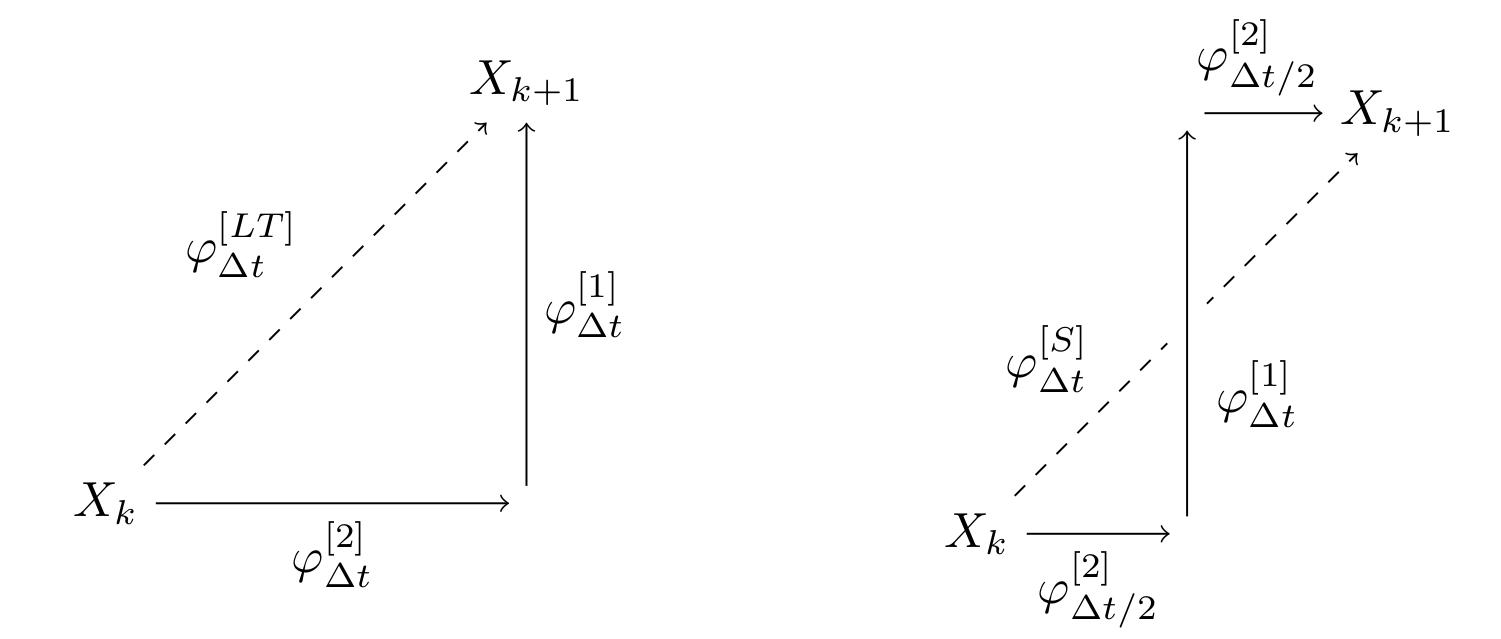
\includegraphics[scale = .2]{figures/strangAndLieTrotter.jpeg}
    \end{center}
    \caption{A diagram of the Lie-trotter- (left) and Strang (right) flows}
    \label{figure:StrangAndLieTrotterPlot}
\end{figure}\\
Although they are quite similar overall, the one-step predictions of the transition densities given by the Strang splitting scheme is proven to be superior to that of LT; compare \cite[Proposition 3.4 and 3.6]{SplittingSchemes}. For this reason, we only consider the Strang splitting scheme. We start by looking at the Strang splitting on a general one-dimensional SDE with additive noise. Later we comment on the possible ways to use this method even for models with multiplicative noise.\\
\textbf{Models with additive noise}\\
General one-dimensional stochastic differential equations with additive noise can be written as
\begin{align}
    \mathrm{d}X_t = b(X_t; \theta)\mathrm{d}t + \sigma\mathrm{d}W_t, \label{eq:generalAdditiveNoiseSDE}
\end{align}
note that we have highlighted the dependence of some parameter, $\theta\in\Theta\subseteq\mathbb{R}^p$ in the drift. When we have additive noise, splitting schemes work by decomposing the process into a linear SDE and a non-linear ODE in the following way
\begin{align}
    \mathrm{d}X_t^{(1)} &= -\beta(\theta)\left(X_t^{(1)} - \mu(\theta)\right)\mathrm{d}t + \sigma \mathrm{d}W_t, &&X_t^{(1)} = x_0, \label{SDE_split}\\
    \mathrm{d}X_t^{(2)} &= N\left(X_t^{(2)}; \theta\right)\mathrm{d}t, &&X_t^{(2)} = x_0, \label{ODE_Split}
\end{align}
where $N$ is some non-linear function that probably depends on the parameters. Evidently, this splitting is not unique, and thus the way we construct the estimator will not be either. However, it turns out that any splitting of (\ref{eq:generalAdditiveNoiseSDE}) yields approximations of the transition densities that are equivalent asymptotically \cite{{SplittingSchemes}}. Yet, our choice might have an impact on the quality for finite samples. Additionally, in practice it is not difficult to imagine that some splittings are numerically more well-behaved than others. So we still have to carefully consider our splitting choice. The one we use for the most part is the heuristic provided in \cite[section 2.3 and 2.5]{SplittingSchemes}. That is, (\ref{SDE_split}) should be constructed as the linearization around the fixed points of the drift. This means, we use $b(X_t, \theta)$ from (\ref{eq:generalAdditiveNoiseSDE}) and solve the following equation
\begin{align}
     b(X_t; \theta) = 0,
\end{align}
in terms of $X_t$. $\mu\left(\theta\right)$ is then defined as the solution. This value is plugged into the derivative of $b(X_t, \theta)$ 
\begin{align}
    \beta\left(\theta\right) = \frac{\partial}{\partial x} b(\mu\left(\theta\right); \theta).
\end{align}
The two components, is put together to construct (\ref{SDE_split}).
Hereafter, (\ref{ODE_Split}) is calculated as the residual of the \ref{eq:generalAdditiveNoiseSDE} and our (\ref{SDE_split}). Recall that in the one dimensional case, the solution with stepsize, $\Delta t$, to the linear SDE is given by the flow
\begin{align}
    \varphi_{\Delta t}^{(1)}(x) = \exp\left(-\beta\left(\theta\right) \Delta t\right)\left(x - \mu\left(\theta\right)\right) + \mu\left(\theta\right) + \xi_{\Delta t}, \label{varphiTheoretical}
\end{align}
with $\xi_{\Delta t}\sim\mathcal{N}\left(0, \Omega_{\Delta t}\right)$. That is, the flow is gaussian with mean and variance
\begin{align}
    \mu_{\Delta t}(x; \theta) &= \exp\left(-\beta\left(\theta\right) \Delta t\right)\left(x - \mu\left(\theta\right)\right) + \mu\left(\theta\right) \label{linearSDEMean}\\
    \Omega_{\Delta t} &= \frac{\sigma^2}{2\beta}\left(1 - \exp\left(-2\beta\left(\theta\right)\Delta t\right)\right), \label{linearSDEVariance}
\end{align}
which we calculated in (\ref{eq:OU_solution}). For our purposes the solution to (\ref{ODE_Split}) exists and is unique; this is ensured by the Picard-Lindelöf theorem \cite[section 2.7]{Srkk2019}, since (\ref{ODE_Split}) is ordinary differential equations that in our case will be sufficiently regular for the assumptions from the theorem to hold. Still, a closed form solution to (\ref{ODE_Split}) might not be possible to get, simply due to the complexity of the ODE. In those cases, we will use the Fourth Order Runge-Kutta method to solve it numerically \cite[p.541 equation (8)]{numericalAnalysis}.  
Nevertheless, we denote the solution with stepsize, $\Delta t$, $\varphi_{\Delta t}^{(2)}$. By figure \ref{figure:StrangAndLieTrotterPlot} the Strang splitting scheme then gives the approximation of the transition density as 
\begin{align}
    X_{t_{i+1}}^{(S)} = \varphi_{\Delta t / 2}^{(2)}\left(\mu_{\Delta t}\left(\varphi_{\Delta t/2}^{(2)}\left(X_{t_{i}}^{(S)}\right); \theta\right) + \xi_{\Delta t} \; ; \theta \right). \label{eq:classicStrangSplitting}
\end{align}
Due to the fact that (\ref{varphiTheoretical}) is gaussian, (\ref{eq:classicStrangSplitting}) is a non-linear transformation of a gaussian variable with the specified mean and variance. So by the density transformation theorem, this flow has the following negative pseudo-loglikelihood 
\begin{align}
    l^{[S]}(\mathbf{x}; \theta) &= -\sum_{i = 0}^{N - 1}\log\left(g\left(\left(\varphi_{\Delta t / 2}^{(2)}\right)^{-1}\left(x_{t_{i+1}}\right); \mu_{\Delta t}\left(\varphi_{\Delta t/2}^{(2)}\left(x_{t_{i}}\right); \theta \right), \Omega_{\Delta t} \right) \right) \nonumber \\
    &- \sum_{i = 0}^{N - 1}\log\left(\frac{\partial}{\partial x}\left(\varphi_{\Delta t / 2}^{(2)}\right)^{-1}\left(x_{t_{i + 1}}\right) \right), \label{eq:Strang_likelihood}
\end{align}
where $t_N$ is the index of the most recent sample in the data. This is the Strang based pseudo-likelihood, and we say that the $\theta$ that minimizes this function is the Strang-based estimator. In (\ref{eq:Strang_likelihood}) $g$ is the density of the gaussian distribution with the specified mean and variance. To get the inverse of the solution to the ODE, we use the property $\left(\varphi_{\Delta t}^{(2)}\right)^{-1} = \left(\varphi_{-\Delta t}^{(2)}\right)$ \cite[Remark below equation (9)]{SplittingSchemes}, and solve ODE corresponding to the right hand side with the Runge-kutta method. Finally, to get the derivative we use Richardson extrapolation. For a function, $f$, the derivative can be approximated as
\begin{align}
    f'(x) = \frac{f(x + h) - f(x - h)}{2h}, \qquad h > 0,
\end{align}
with an error that is $\mathcal{O}(h^2)$. It is possible to repeatedly use Richardson extrapolation to get even higher-orders of precision. However, for our purposes this simple approximation suffices.
\\\\
\textbf{Models with multiplicative noise}\\
As we noted, we require additive noise in the models. This is, because the method hinges on that we an Ornstein-Uhlenbeck process in (\ref{SDE_split}). For many models that interest us, this, of course, not be the case in itself. But all the models we consider are reducible, and as such we can transform the processes with the lamperti-transform (\ref{eq:lampertiDefinition}) and do the estimation on the resulting SDE in the exact manner as we just described. This is the method introduced in \cite{SplittingSchemes}, for which there exist theoretical results on the accuracy of the transition density.\\
Still, we consider different options. As an alternative, we use the same splitting philosophy, but leave the noise as it is. This of course means that the linear SDE inherits the multiplicative noise. Other methods for approximating such methods exist. The one we use is Kessler's method; this method assumes a gaussian transition density, but uses the true conditional mean- and variance \cite[equation (1.7)]{Kessler1997}. Even still, there is another possibility. In a few cases there exists other closed form solutions to linear stochastic differential equations than the one with additive noise. This splitting strategy avoids using the Lamperti-transform, while avoiding approximating any solution to an SDE. Although, the last two types of splittings are not central to the thesis, we still illustrate. Derivation for the latter option can for instance be seen in (\ref{meanrevertingGBMSplit1}). Note that in this example, we must use a different splitting than the heuristic provided by \cite[section 2.3 and 2.5]{SplittingSchemes}, because the solution of the stochastic differential equation in the example only exists on closed-form, whenever $\mu(\lambda) = 0$. We would have to be quite fortunate to have the fixed point equal 0; thus this splitting strategy rarely aligns with the heuristic from the paper.
\subsubsection{Approximately Optimal Martingale Estimation Equations}\label{subsubsec:approximatelyOptimalMartingaleEstimationEquation}
Other than the strang splitting, we also estimate the parameters by means of approximately optimal martingale estimation functions (AOMEF). As a means of estimation these are conceptually different from what we have done thus far; with them our aim is not to approximate the transition density, but instead construct functions where the estimator is defined as a solution to a system of equations similarly to how a score function (\ref{eq:transitionScore}) normally is used.\\
Not surprisingly, AOMEF's are based on the notion of an martingale estimaton equation. The theory behind these is quite involved measure-theoretically, for which reason we only summarize the most important ideas in their construction. We imagine that we want to estimate the parameters, $\theta\in \Theta \subseteq \mathbb{R}^p$ and $\sigma$, in a one-dimensional stochastic differential equation such as (\ref{eq:SDEInference}); and say that the solution to this equation has state space, $D\subseteq \mathbb{R}$. Furthermore, let $p(x, y, \Delta t; \theta)$ be the transition density of $X_{t+\Delta t}$ given $X_t$, evaluated at the point $y$. Then a martingale estimation function is 
\begin{align}
    G_N(\theta) = \sum_{i = 1}^N g(X_{t_{i - 1}}, X_{t_i}, \Delta t; \theta), \label{eq:estimationEquation}
\end{align}
where $g$ is some function such that
\begin{align}
    \int_{D} g(x, y, \Delta t; \theta)p(x, y, \Delta t; \theta)\mathrm{d}y = 0. \label{eq:martingaleProperty}
\end{align}
In other words, $G_N$ is a martingale w.r.t. the filtration $\mathcal{F}_n = \sigma\left(X_{t_i}; i \leq n\right)$. \cite[p. 11]{StatisticalMethodsForSDE} establishes that an example of such an equation are the score equations; this is easily seen by inserting (\ref{eq:transitionScore}) in (\ref{eq:martingaleProperty}). That is the martingale equations can be seen as a generalization of the score equation. Now, we know that the solving the score equation yields the maximum likelihood estimator; an estimator with many desirable properties. Thus, we are interested in picking a function $g$ satisfying (\ref{eq:martingaleProperty}) that is optimal in the sense that it approximates the score well. We do this by taking a collection of real valued functions $h = (h_1, \dots, h_m)^\top$, where each individual function satisfies (\ref{eq:martingaleProperty}) and choose $g$ in (\ref{eq:estimationEquation}) so
\begin{align}
    G_N(\theta) = \sum_{i = 1}^N a\left(X_{t_i}, \Delta t, \theta \right)h(X_{t_{i - 1}}, X_{t_i}, \Delta t; \theta), \label{eq:estimationEquationWeight},
\end{align}
where $a$ is a $p\times m$-matrix that is a function that (\ref{eq:estimationEquationWeight}) is integrable w.r.t. $P_\theta$. Therefore (\ref{eq:estimationEquationWeight}) is a martingale, because the $h_j$ satisfy (\ref{eq:estimationEquation}). The $h$-functions are often chosen such that
\begin{align}
    h_j = f_j(X_i, \Delta t) - \mathbb{E}_\theta\left[f_j(X_i)| X_{t_{i - 1}} = x_{t_{i - 1}}\right].
\end{align}
The specific $h$-functions, we consider, are
\begin{align}
    h_1(x,y, \Delta t; \theta) &= y - \mathbb{E}_\theta\left[X_{t_i + \Delta t} \middle| X_{t_{i}} = x\right] \\
    h_2(x,y, \Delta t; \theta) &= \left(y - \mathbb{E}_\theta\left[X_{t_i + \Delta t} \middle| X_{t_{i}} = x\right]\right)^2 - \mathrm{Var}\left[X_{t_i + \Delta t} \middle| X_{t_{i}} = x\right],
\end{align}
For typographical reasons denote the conditional mean and -variance, $F$ $\Phi$, respectively, in the following.
 We use the estimation function based on the quasi-score function of a gaussian transition density \cite[equation (1.28)]{StatisticalMethodsForSDE}. This corresponds to using the weight matrix
 \begin{align}
    \left(\frac{\frac{\partial}{\partial\theta}F(\Delta t, x;\theta)}{\Phi\left(\Delta t, x; \theta\right)} , \frac{\frac{\partial}{\partial\theta}\Phi(\Delta t, x;\theta)}{2\Phi^2(\Delta t, x;\theta)\Delta t} \right),
\end{align}
in (\ref{eq:estimationEquationWeight}) along with the $h$-functions from before. It turns out that for small enough $\Delta t$, these weights are a good approximation of the actual optimal weights \cite[equation (1.32)]{StatisticalMethodsForSDE}, which can be much more complex. Finally, by \cite[lemma 1.10]{StatisticalMethodsForSDE} the weight can be simplified to
\begin{align}
    \left(\frac{\frac{\partial}{\partial\theta}b(\Delta t, x;\theta)}{\sigma^2\left(\Delta t, x; \theta\right)} , \frac{\frac{\partial}{\partial\theta}\sigma^2(\Delta t, x;\theta)}{2\sigma^4(\Delta t, x;\theta)\Delta t} \right),
\end{align}
This gives us the estimation equations for one-dimension stochastic differential equations, which \cite[Example 1.11]{StatisticalMethodsForSDE} arrives at
\begin{align}
    G_N^{\circ} &= \sum_{i = 1}^N 
    \left(
        \frac{\frac{\partial}{\partial\theta} b\left(X_{t_{i-1}};\theta\right)}{\sigma^2\left(X_{t_{i-1}};\theta\right)}
    \right) \left(X_{t_{i}} - \mathbb{E}\left[X_{t_{i}} \middle| X_{t_{i-1}} = x\right]\right) \nonumber \\
    &+ \frac{\frac{\partial}{\partial\theta}\sigma^2\left(X_{t_{i-1}}; \theta\right)}{2\sigma^4\left(X_{t_{i - 1}}; \theta\right)\Delta t}\left(\left(X_{t_{i}} - \mathbb{E}\left[X_{t_{i}} \middle| X_{t_{i-1}} = x\right]\right)^2 - \textrm{Var}\left[X_{t_{i}} \middle| X_{t_{i-1}} = x\right]\right),\label{eq:approximatelyOptimalMartingale}
\end{align}
and even with the numerous assumptions and simplifications made thus far, this approximately optimal martingale estimation equation still gives a consistent estimator of $\theta$ \cite[p.19]{StatisticalMethodsForSDE}. In appendix \ref{sec:AppendixEstim} we derive estimators that are based on these methods for two of the pearson diffusions.

\subsection{Numerical Optimization in \code{R}}
Numeric optimization is central in applications of machine learning and statistics. In this section, we mention the methods used in the thesis and some motivation for the choices that was made. Also, we introduce a numerical Strang-based negative log-likelihood based on the heuristics of \cite{SplittingSchemes}, where the user only needs to specify the drift of the lamperti-transformed SDE.
\subsubsection{General optimization and implementation}
For each part of the process i.e. before and after ramping begins, we optimize a bit differently. Because of this, we have implemented two wrappers around {stats::optim} \cite{Rlang}. Each of which is implemented such that they can be invoked with any likelihood function, we have implemented for that part. In addtion, we allow any valid \code{optim}-argument to be called in both wrappers. This is especially useful, because the arguments to \code{optim} can vary depending on the specific algorithm, one wishes to use. Also, since \code{optim} uses an ellipsis, our wrappers does too. That is, our wrapper can pass on any argument directly onto \code{optim}. This is for example useful, if we have objective functions with special arguments that we would like to pass onto it in the optimization.\\
Still, the wrapper obviously has to have a couple of default arguments to make it easier to use. For instance, both parts use the built-in BFGS optimization algorithm, due to its robustness. Though, as said we could specify any other optimization algorithm implemented in \code{optim} during the call.\\ For the dynamic part, we need to provide the values for $\alpha_0, \mu_0, \sigma$. This the ellipsis seemingly allows us to do. Of course, the values we pass on here are the estimated values for these from the stationary part of the processes. In addition, the optimizer of the dynamic part dynamically chooses to estimate the $\nu$-parameter dependending on the dimension of the initial values that are provide to it. If the dimension is two, we implicitly assume $\nu = 1$, while a dimension of three allows the optimizer to estimate it. With regards to the numerical stability of the implementations we do a few things. Firstly, terms including $\exp\left(x\right) - 1$ or its additive inverse show up in many of our formulas. This is for instance the case in (\ref{linearSDEVariance}). As the arguments for the exponential function often is quite close to zero in these applications, we need to take care in order to avoid catastrophic cancellation. Luckily, others have had this problem before us, and we make use of the \code{base::expm1} method in \code{R}, which calls the C-function of the same name \cite{cppreference_expm1} - a method optimized for this very problem. If we do not do this, our program might crash or give misleading estimates. In the case of (\ref{linearSDEVariance}) for instance, we risk having a variance of zero. While the methods in \code{R} that use the gaussian distribution allow the use of this degenerate distribution, we are of course not interested in such a transition density.
\subsubsection{A numerical Strang method in \code{R}}
In this section, we briefly describe an almost entirely numerical Strang splitting scheme based estimator with our usual splitting philosophy. The algebra required in the derivations of this method to obtain the necessary elements can be quite cumbersome. We have already limited the amount of errors we can do somewhat by relying on the Fourth-Order Runge-kutta method to solve ODE's in some of the versions of the Strang splitting. Limiting the amount of computations further could have an advantage; however it is naturally more difficult to implement. Nevertheless, As of the current implementation, we are at the amount of automation, we we only need to derive two things ourselves: The Lamperti-transform and the drift of the SDE that comes as a result of it. Passing these onto our wrapper for the optimizer and we optimize the Strang-based likelihood. \\
The method works the same as the less automated versions with regards to solving the ODE's. However, the construction of (\ref{SDE_split}) and (\ref{ODE_Split}) is different. The latter is of course just computed as the residual of lampert transformed drift that we pass to the method and the linear SDE. The linear SDE is constructed as the linearization around the fixed point of the drift. The fixed point is found using the method \code{nleqslv::nleqslv}, which find zeroes with Newton's method \cite{nleqslv}. We then find the derivative of the drift numerically with \code{numDeriv::grad} \cite{numDeriv}. We plug the fixed point into this function to get the the slope of the linearization.
\subsection{Model assessment}
For this part, we briefly introduce the metrics used for evaluating the quality of our estimators in a simulation setting. Additionally, we show the method that we use to diagnose the fit of a particular method to data, and how we contruct confidence intervals for the estimators.
\subsubsection{Diagnostics and confidence intervals}
When we are in a simulation setting, we assess the precision of our estimation methods using the mean of the absolute relative error over a number of simulations, $M$, each with sample size, $N$. This is for the $i$th-coordinate in our parameter vector defined as
\begin{align}
    \mathrm{ARE}\left(\theta_N^{(i)}\right) = \frac{1}{M}\sum_{j = 1}^M\frac{\left|\theta_{N,j}^{(i)} - \theta_{0,j}^{(i)}\right|}{\theta_{0,j}^{(i)}}.
\end{align}
Of course, we are not able to calculate this quantity when we do not have access to the ground-truth parameters. Also, we cannot use regular residuals to diagnose the fit, as each data point have different distributions depending on the previous point. Instead, we assess the fit qua so-called uniform residuals. These are constructed using the transition density, $p_\theta(x|\Delta t, x_0)$. Though, as is quite clear by now, this is rarely something we can compute. However, we can use the approximation given from the Strang scheme in its stead. This also gives us an approximation for the conditional distribution function, $F_\theta(x|\Delta t, x_0)$, and as $F_\theta(X_{t_{i}}|\Delta t, X_{t_{i - 1}})\sim \mathrm{Unif}(0,1)$ if $X_{t_{i}}|X_{t_{i - 1}} \sim p_\theta$. It is sometimes difficult to detect outliers in the uniform distribution, so we transform the quantity with the quantile function of the standard gaussian distribution, such that we by the quantile transformation theorem have samples that are standard gaussian. The fit can then be diagnosed by means of ordinary Q-Q plots.\\
As the approximately optimal martingale estimation functions approximate the score function, we do not have any approximation of the transition density here and cannot use uniform residuals. Even still with some creativity, we can do diagnostics, but only of the square-root process. If we let $X_t$ to be governed by the square-root process, then
\begin{align}
    Y_{t_{i + 1}} := \frac{4\beta}{\sigma^2\left(\exp\left(-\beta \Delta t\right) - 1\right)}X_{t_{i + 1}}
\end{align}
has transition density of a non-central $\chi^2$-distribution with $\frac{4\beta\mu}{\sigma^2}$ degrees of freedom with non-centrality parameter $Y_{t_k}\exp\left(-\beta \Delta t\right)$ \cite[Equation (5.68)]{Srkk2019}. For the other diffusions, we do not have an analagous property to exploit, and we may only assess the score function based estimators by ensuring that the estimates are consitent with methods based on the transition density; for which we use the uniform residuals. Finally, we obviously have no hope of knowing the distribution of our estimators. Therefore to get an idea of our uncertainty of them, we use parametric bootstrap. That is, we estimate on the data with a specific model and then sample from that model repeatedly using the parameters estimated on the real data. The empiric distribution of the estimates achieved in this way then gives us the quantiles etc. for our estimator.